\section{Results}
\label{sec:results}
\subsection{Coherence Misses}
Figure~\ref{fig:coherence} depicts the reduction in coherence misses with the
MESHI protocol. The coherence misses include both: (1) Loads to data found in
the \emph{INV} state in the cache and (2) Stores to data found in the cache in a
shared or invalid state. As expected, as the amount of approximation increases the coherence miss
count reduces. What is interesting is that in most cases the drop in coherence
misses is disproportionate with the fraction of "Big" writes. For example,
treating 20\% of all writes as "Big" reduces the number of coherence misses by
close to 97\% in most of the workloads that we evaluate here. The 25\% point in
\emph{streamcluster} seems to be an anomaly here.  
\begin{figure}[t] \centering 
%\vspace{-0.4cm}
%\vspace{-0.1cm}
\centering
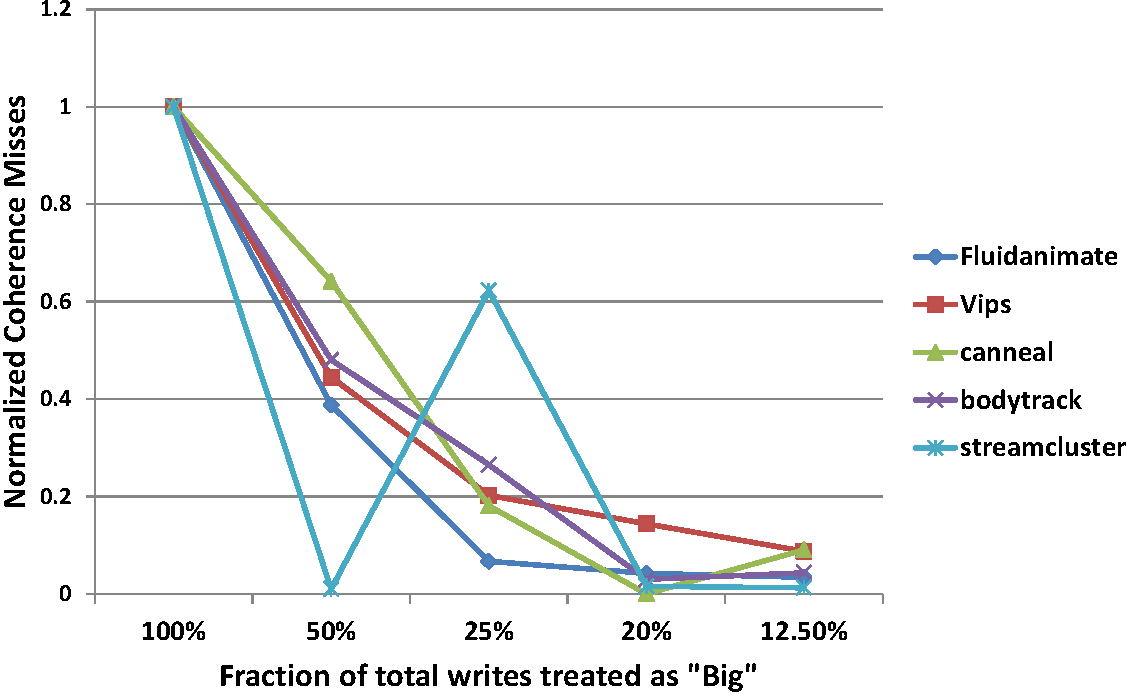
\includegraphics[width=0.49\textwidth]{figures/coherence_misses-crop.pdf}
\caption{Reduction in Coherence Misses.}
\label{fig:coherence}
\end{figure}

\subsection{Invalidate Traffic}
Figure~\ref{fig:invalidates} depicts the change in invalidate traffic as a
result of the approximate coherence protocol. We define the number of
invalidates the number of messages to other caches to invalidate cache lines
because of the cache coherence protocol. We observe the impact of
approximation varies across different workloads. For example, \emph{bodytrack}
benefits the least, with the reduction in invalidate traffic being only about
20\% even with aggressive approximation. Whereas \emph{vips} benefits a lot
more commensurately with the approximation. We attribute this difference to the
amount of sharing between different threads at any given time, where \emph{vips}
most likely has a lot more cores sharing a piece of data during an write
operation than \emph{bodytrack}.  

\begin{figure}[t] \centering 
%\vspace{-0.4cm}
%\vspace{-0.1cm}
\centering
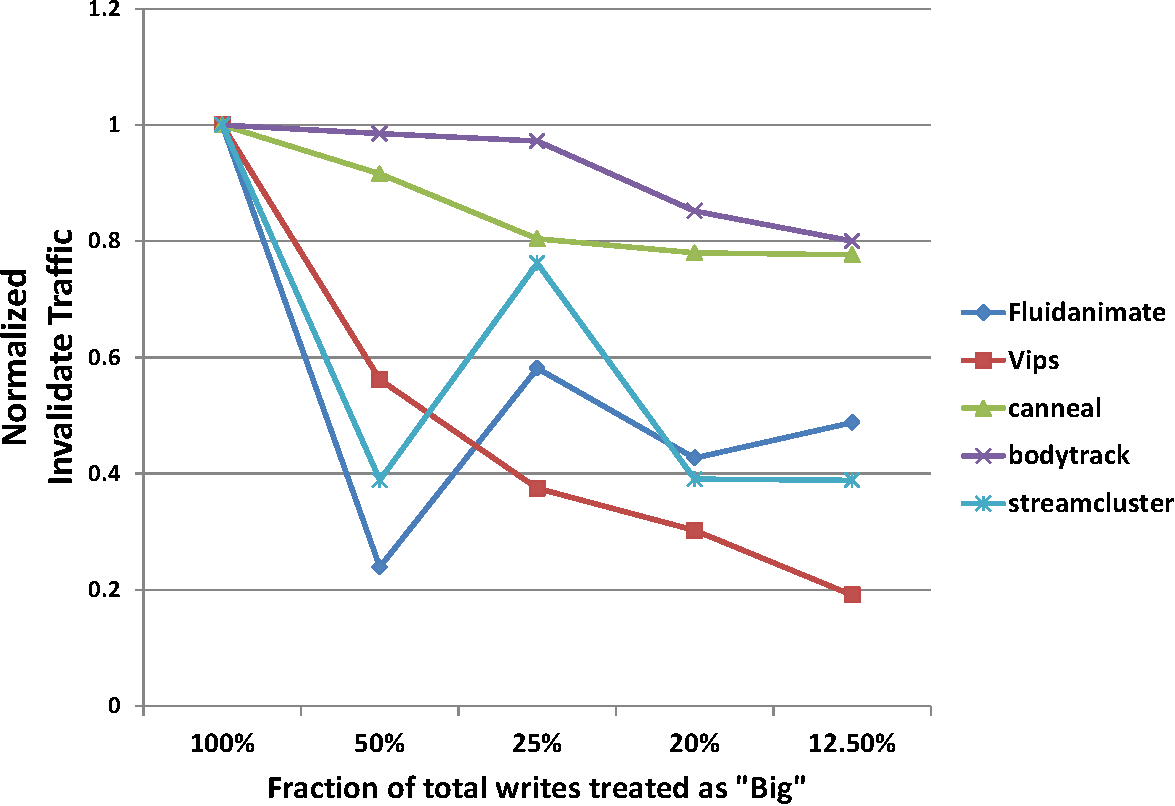
\includegraphics[width=0.49\textwidth]{figures/Invalidates-crop.pdf}
\caption{Reduction in Invalidate Traffic.}
\label{fig:invalidates}
\end{figure}

\subsection{Directory Lookups}
Figure~\ref{fig:lookups} depicts the number of the directory lookups as we vary
the extent
of approximation in the coherence protocol. Again we see a huge drop in the
number of directory lookups at a certain point (20\%) in most of the workloads.
Upto that point the reduction is more on-par with the fraction of "Big" writes.
The "M" state allows for a lot more silent updates than before.  

\begin{figure}[t] \centering 
%\vspace{-0.4cm}
%\vspace{-0.1cm}
\centering
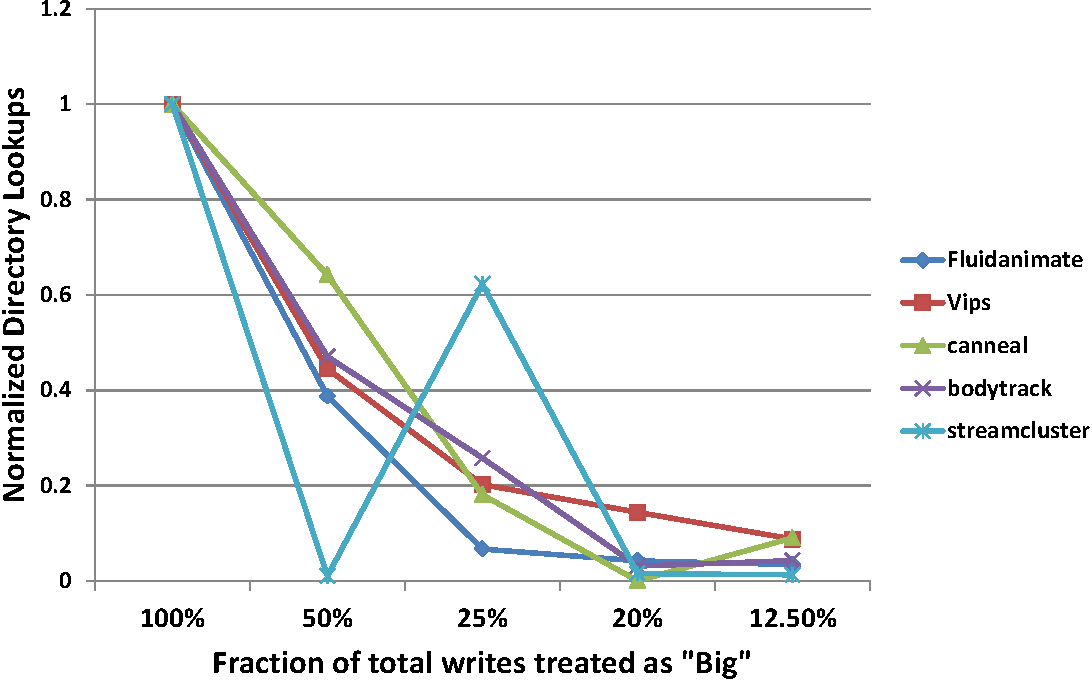
\includegraphics[width=0.49\textwidth]{figures/Lookups-crop.pdf}
\caption{Reduction in Directory Lookups.}
\label{fig:lookups}
\end{figure}

\subsection{Writebacks}
Figure~\ref{fig:writeupdates} shows the number of cache lines that were shuttled
back and forth across cores as a result of data sharing. As expected,
approximation certainly provides a reduction in the number of cache lines that
ping-pong between different cores. The extent again varies across the different
workloads, with \emph{Canneal} and \emph{Bodytrack} benefitting the most.  
 
\begin{figure}[t] \centering 
%\vspace{-0.4cm}
%\vspace{-0.1cm}
\centering
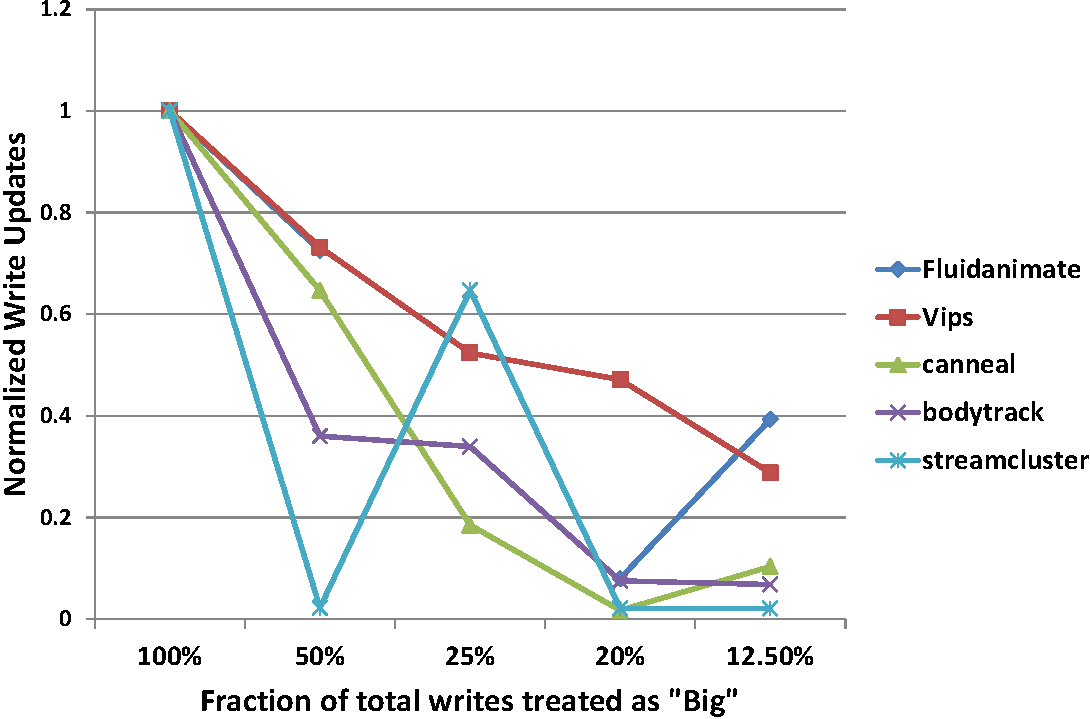
\includegraphics[width=0.49\textwidth]{figures/WriteUpdates-crop.pdf}
\caption{Reduction in Writebacks.}
\label{fig:writeupdates}
\end{figure}

